% XeLaTeX, two passes. Standalone folder: images/ and data/ travel with main.tex.
\RequirePackage{fix-cm}
\documentclass[aspectratio=169,10pt]{beamer}
\usepackage{fontspec}
\setsansfont{Arial}
\setmainfont{Arial}
\usefonttheme{professionalfonts}
\usepackage{amsmath,booktabs,array,colortbl,graphicx,pgfplots}
\pgfplotsset{compat=1.18}
% Lecture-style theme: white canvas, gray title band and blue footer.
\definecolor{Navy}{HTML}{12366D}
\definecolor{Blue}{HTML}{1458B5}
\definecolor{MidBlue}{HTML}{4D84C6}
\definecolor{Teal}{HTML}{1458B5}
\definecolor{Orange}{HTML}{4D84C6}
\definecolor{Muted}{HTML}{5E6672}
\definecolor{Light}{HTML}{E8F0FA}
\definecolor{TitleBand}{HTML}{F2F2F2}
\setbeamercolor{normal text}{fg=black,bg=white}
\setbeamercolor{frametitle}{fg=Blue,bg=TitleBand}
\setbeamercolor{structure}{fg=Blue}
\setbeamercolor{alerted text}{fg=Blue}
\setbeamercolor{foot author}{fg=white,bg=Blue}
\setbeamercolor{foot course}{fg=Blue,bg=TitleBand}
\setbeamercolor{foot title}{fg=Navy,bg=Light}
\setbeamercolor{foot page}{fg=Blue,bg=TitleBand}
\setbeamerfont{frametitle}{size=\fontsize{14}{17}\selectfont,series=\mdseries}
\setbeamerfont{footline}{size=\fontsize{7}{8.5}\selectfont}
\setbeamertemplate{navigation symbols}{}
\setbeamertemplate{itemize item}[ball]
\setbeamertemplate{itemize subitem}[circle]
\setbeamersize{text margin left=8mm,text margin right=8mm}
\setbeamertemplate{frametitle}{%
  \nointerlineskip
  \begin{beamercolorbox}[wd=\paperwidth,sep=0pt,leftskip=4mm,rightskip=4mm]{frametitle}
    \vbox{}\vskip0.6mm
    \usebeamerfont{frametitle}\strut\insertframetitle\strut\par
    \vskip0.6mm
  \end{beamercolorbox}%
}
\newcommand{\insertpaperreference}{}
\newcommand{\paperreference}[1]{\gdef\insertpaperreference{#1}}
\setbeamertemplate{footline}{%
  \leavevmode\hbox{%
    \begin{beamercolorbox}[wd=.12\paperwidth,ht=2.3mm,dp=0.6mm,center]{foot author}%
      \usebeamerfont{footline}Nhóm 2
    \end{beamercolorbox}%
    \begin{beamercolorbox}[wd=.16\paperwidth,ht=2.3mm,dp=0.6mm,center]{foot course}%
      \usebeamerfont{footline}Xử lý ảnh
    \end{beamercolorbox}%
    \begin{beamercolorbox}[wd=.60\paperwidth,ht=2.3mm,dp=0.6mm,center]{foot title}%
      \usebeamerfont{footline}\fontsize{6.5}{7.5}\selectfont\insertpaperreference
    \end{beamercolorbox}%
    \begin{beamercolorbox}[wd=.12\paperwidth,ht=2.3mm,dp=0.6mm,center]{foot page}%
      \usebeamerfont{footline}\insertframenumber\ /\ \inserttotalframenumber
    \end{beamercolorbox}%
  }%
}
\setbeameroption{hide notes}
\setlength{\parskip}{4pt}
\graphicspath{{images/}}
\newcommand{\captionnote}[1]{\par\vspace{1mm}{\fontsize{7}{8.5}\selectfont\color{Muted}#1\par}}
\newcommand{\takeaway}[1]{\par\vspace{2mm}{\color{Teal}\bfseries#1\par}}
\newcommand{\smalltable}{\fontsize{9}{11}\selectfont\renewcommand{\arraystretch}{1.25}}
\pgfplotsset{slideplot/.style={
  width=10.5cm,height=5.25cm,
  axis lines=left,axis line style={Muted!50},
  tick label style={font=\scriptsize,color=Muted},
  label style={font=\small},
  legend style={font=\scriptsize,draw=none,fill=none},
  ymajorgrids=true,grid style={Light},
  tick align=outside,clip=false,
  every axis plot/.append style={line width=1.2pt,mark size=2pt}
}}
\hypersetup{pdftitle={Xử lý ảnh thiếu sáng cho nhận dạng biển báo giao thông},pdfauthor={Nhóm 2, Đại học Phenikaa}}
\begin{document}

% 01
\paperreference{}
\begin{frame}{Bài tập lớn môn Xử lý ảnh}
\begingroup\setlength{\parskip}{2pt}
\begin{columns}[T,onlytextwidth]
\column{0.83\textwidth}
{\small ĐẠI HỌC PHENIKAA\par TRƯỜNG CÔNG NGHỆ THÔNG TIN PHENIKAA}
\column{0.12\textwidth}
\includegraphics[width=1.2cm]{phenikaa.jpg}
\end{columns}
\par\vspace{4mm}
{\fontsize{18}{22}\selectfont\bfseries
Khảo sát ảnh hưởng của xử lý ảnh\par
đến hiệu năng nhận dạng biển báo\par
giao thông trong điều kiện thiếu sáng\par}
\par\vspace{2mm}
{\small\textbf{Giảng viên hướng dẫn:} TS. Nguyễn Ngọc Giang\par}
{\fontsize{8}{10}\selectfont\textbf{Nhóm 2}\par
\begin{tabular}{@{}lll@{}}
Kiều Thị Thu Trang & 24100093 & 24100093@st.phenikaa-uni.edu.vn\\
Trần Minh Sang & 24100012 & 24100012@st.phenikaa-uni.edu.vn\\
Ngô Quang Thiện & 24102651 & 24102651@st.phenikaa-uni.edu.vn
\end{tabular}\par}
{\scriptsize GTSRB \qquad ResNet-18 \qquad Tháng 10/2026}
\par\vspace{1mm}{\fontsize{8}{10}\selectfont Demo: \url{https://image-preprocessing.techvi.io.vn}}
\endgroup
\note{Thời lượng khoảng 30 giây. Giới thiệu tên đề tài và thành viên. Nhấn mạnh đối tượng khảo sát là các phép xử lý ảnh, còn ResNet-18 đóng vai trò bộ nhận dạng cố định để kiểm chứng. }
\end{frame}

% 02
\paperreference{}
\begin{frame}{1.1. Mục tiêu: xử lý ảnh có giúp nhận dạng đúng hơn?}
\textbf{Vấn đề}\par
Ảnh thiếu sáng có thể bị tối và nhiễu, khiến mô hình nhầm biển báo.
Ảnh sau xử lý dễ nhìn hơn chưa chắc được nhận dạng đúng hơn.
\par\vspace{3mm}
\textbf{Nhóm kiểm tra những gì?}
\begin{itemize}
\item So sánh 7 phương pháp tăng cường ảnh và 3 bộ lọc khử nhiễu.
\item Thử khử nhiễu trước hoặc sau Gamma/CLAHE.
\item Đo mức gần ảnh gốc và độ chính xác nhận dạng bằng ResNet-18.
\end{itemize}
\par\vspace{2mm}
\textbf{Phạm vi:} ảnh đã cắt vùng biển báo GTSRB, 43 lớp; độ tối và nhiễu
được tạo bằng công thức. Chưa kiểm tra video hay camera ban đêm thực.
\takeaway{Mục tiêu là giữ thông tin giúp nhận dạng, không chỉ làm ảnh sáng hơn.}
\note{Mở bằng câu hỏi nghiên cứu. Tăng cường gồm điều chỉnh độ sáng, tương phản; khảo sát còn có khử nhiễu và thứ tự kết hợp. Nguồn: báo cáo chương 1 và chương 6.}
\end{frame}

% 03
\paperreference{\href{https://doi.org/10.1109/IJCNN.2011.6033395}{Stallkamp et al., IJCNN 2011}}
\begin{frame}{1.2. GTSRB: chia dữ liệu để tránh học trùng ảnh}
\begin{columns}[T,onlytextwidth]
\column{.39\textwidth}
\textbf{43 lớp biển báo Đức}\par\vspace{2mm}
\smalltable
\begin{tabular}{lr}\toprule
Tập dữ liệu & Số ảnh\\\midrule
Huấn luyện & 31.350\\
Chọn cấu hình & 7.829\\
Cách ly & 30\\
Kiểm tra cuối & 12.630\\\bottomrule
\end{tabular}
\column{.57\textwidth}
\textbf{Mỗi tập có vai trò riêng}\par
Train: học trọng số mô hình.\par
Validation: chọn mô hình và tham số xử lý.\par
Test: đo kết quả cuối, không dùng chọn tham số.
\par\vspace{2mm}
\textbf{Track là chuỗi ảnh cùng một biển thực tế.}\par
Giữ cả chuỗi trong cùng train hoặc validation để tránh ảnh gần giống nhau xuất hiện ở cả hai tập.
\end{columns}
\takeaway{Cách ly cả track chứa ảnh trùng test: 30 ảnh, trong đó 8 ảnh trùng pixel.}
\captionnote{Giữ nguyên tập test chính thức. Nhãn đúng và tọa độ vùng biển báo có sẵn trong GTSRB.}
\note{Tổng ảnh training nguồn là 39.209; 31.350 cộng 7.829 cộng 30. Kiểm tra trùng dựa trên pixel, không phải tên file. Không suy diễn rằng mọi tương quan trong test đã bị loại. Nguồn: src/data.py; báo cáo mục 2.1 và 2.2.}
\end{frame}

\paperreference{}
\begin{frame}{1.3. Chuẩn bị vùng biển báo trước khi tạo suy giảm}
\begin{enumerate}
\item \textbf{Cắt vùng biển báo (ROI)} theo tọa độ có sẵn trong dữ liệu.
Bỏ phần ngoài vùng cần nhận dạng.
\item \textbf{Mở rộng lề 5\% mỗi phía} theo chiều rộng/cao của ROI,
để giữ đường viền và một ít ngữ cảnh.
\item \textbf{Đổi sang RGB và resize về $64\times64$ pixel.}
Resize co/giãn vùng ảnh, không phải cắt thêm ảnh.
\item \textbf{Chia giá trị pixel cho 255:} chuyển từ $[0,255]$ sang $[0,1]$
để công thức và mức nhiễu dùng cùng thang đo.
\end{enumerate}
\takeaway{Tạo nhiễu sau resize để kiểm soát nhiễu ở cùng kích thước đầu vào.}
\captionnote{Nội suy có thể làm mất nét nhỏ. Thiết kế này phục vụ so sánh có kiểm soát, không mô phỏng đầy đủ camera.}
\note{Ví dụ ROI rộng 100, cao 60 thì thêm khoảng 5 pixel mỗi bên trái/phải và 3 pixel mỗi bên trên/dưới. Lề được chặn tại biên ảnh. Resize song tuyến tính có thể đổi tỷ lệ và làm mềm nét; phóng lên 224 không tái tạo chi tiết. Nguồn: báo cáo mục 2.2, 2.3.3; src/data.py.}
\end{frame}

% 04
\paperreference{}
\begin{frame}{2.1. Tạo ảnh thiếu sáng theo bốn bước nối tiếp}
\textbf{$X$: pixel ảnh gốc đã chuẩn hóa về $[0,1]$.}
\par\vspace{3mm}
\renewcommand{\arraystretch}{1.5}
\begin{tabular}{@{}p{3.7cm}p{3.5cm}p{6.0cm}@{}}
\textbf{Bước} & \textbf{Công thức} & \textbf{Ý nghĩa đầu ra}\\\midrule
1. Làm tối bằng Gamma & $U=X^{\gamma_d}$ & $U$: ảnh tối, chưa thêm nhiễu.\\
2. Thêm Poisson & \shortstack[l]{$K\sim\mathrm{Poisson}(pU)$\\$V=K/p$} & $V$: đã tối và có nhiễu phụ thuộc tín hiệu.\\
3. Cộng Gaussian & $W=V+\varepsilon$ & $W$: có thêm nhiễu cộng; $\varepsilon\sim\mathcal N(0,\sigma_n^2)$.\\
4. Chặn miền giá trị & $Y=\mathrm{clip}(W,0,1)$ & Giá trị âm thành 0, vượt 1 thành 1.\\
\end{tabular}
\takeaway{$X\rightarrow U\rightarrow V\rightarrow W\rightarrow Y$: cùng một pixel qua từng bước.}
\captionnote{Poisson là lấy mẫu ngẫu nhiên, không phải tính xác suất. Với cùng $U>0$, phương sai của $V$ bằng $U/p$.}
\note{Công thức áp dụng riêng cho từng giá trị kênh màu. Gamma lớn hơn 1 làm tối trên miền chuẩn hóa. Poisson mô tả dao động phụ thuộc tín hiệu; Gaussian thêm dao động có sigma cố định. Cả hai cùng xuất hiện trong ảnh cuối. Đây là mô hình tổng hợp. Nguồn: src/degradation.py; báo cáo mục 2.3.}
\end{frame}

\paperreference{}
\begin{frame}{2.2. Ba mức suy giảm đều có độ tối và cả hai loại nhiễu}
\begin{columns}[c,onlytextwidth]
\column{.65\textwidth}
\includegraphics[width=\linewidth,height=4.7cm,keepaspectratio]{degradation.png}
\column{.32\textwidth}
\smalltable
\begin{tabular}{lrrr}\toprule
Mức & $\gamma_d$ & $p$ & $\sigma_n$\\\midrule
Nhẹ & 1,5 & 120 & 0,005\\
Vừa & 2,2 & 60 & 0,010\\
Nặng & 3,0 & 30 & 0,020\\\bottomrule
\end{tabular}
\par\vspace{3mm}
\normalsize
$\gamma_d$ tăng: ảnh tối hơn.\par
$p$ giảm: Poisson mạnh hơn ở cùng tín hiệu.\par
$\sigma_n$ tăng: Gaussian mạnh hơn.
\end{columns}
\takeaway{Mỗi ảnh nhẹ/vừa/nặng đều đã qua toàn bộ bốn bước, không phải một bước riêng.}
\captionnote{Histogram là phân bố số pixel theo cường độ. Cùng một mẫu validation, noise seed 101.}
\note{Hàng ảnh clean là tham chiếu trước suy giảm. Cả ba ảnh còn lại đều có đủ Gamma, Poisson và Gaussian. Thay đổi cả ba tham số nên chênh lệch giữa các mức không chỉ do độ tối. Hình: report/slides/images/degradation.png; nguồn số: configs/resnet18.json.}
\end{frame}

% 05
\paperreference{\href{https://ntrs.nasa.gov/api/citations/19990005051/downloads/19990005051.pdf}{Jobson et al., IEEE TIP 1997}}
\begin{frame}{3.1. Cơ chế tăng cường ảnh: bốn phương pháp truyền thống}
\smalltable
\begin{tabular}{@{}p{2.4cm}p{11.3cm}@{}}\toprule
\textbf{Phương pháp} & \textbf{Cơ chế chính và công thức}\\\midrule
Gamma & $\widehat X=Y^\alpha$, $0<\alpha<1$: nâng cường độ vùng tối. Cùng một số mũ cho toàn ảnh; $\alpha$ nhỏ làm sáng mạnh hơn.\\[4pt]
HE & Dùng histogram toàn kênh sáng để tính tỷ lệ tích lũy $C(k)$, rồi đổi mức sáng:
$T(k)=\mathrm{round}\!\left[255\frac{C(k)-C_{\min}}{1-C_{\min}}\right]$.\\[4pt]
CLAHE & Chia kênh sáng thành các ô; giới hạn cột histogram quá cao, tính ánh xạ HE từng ô rồi nội suy giữa các ô. Hạn chế khuếch đại tương phản quá mức.\\[4pt]
MSR (Retinex) & Ước lượng chiếu sáng bằng ảnh mờ ở nhiều mức:\newline
\mbox{$r=\frac1S\sum_s[\log(Y+\epsilon)-\log(G_{\sigma_s}*Y+\epsilon)]$}. Đưa $r$ về $[0,1]$.\\\bottomrule
\end{tabular}
\par\vspace{3mm}
{\small $Y$: ảnh đầu vào; $\widehat X$: ảnh sau xử lý; $k$: mức sáng; $C_{\min}$: giá trị tích lũy khác 0 đầu tiên.\par
$G_{\sigma_s}*Y$: ảnh làm mờ; $S$: số mức làm mờ; $\epsilon$: hằng số nhỏ tránh $\log0$.}
\captionnote{HE/CLAHE xử lý trên kênh độ sáng Y. MSR là bản giản lược; bốn phương pháp này không cần huấn luyện.}
\note{HE dùng CDF chuẩn hóa; ảnh hằng xử lý riêng. MSR còn chuẩn hóa phân vị 1--99 phần trăm. Y trong bảng là ảnh đầu vào; Y trong không gian YCrCb là kênh độ sáng. Nguồn: src/enhancement.py; báo cáo mục 3.2--3.5.}
\end{frame}

\paperreference{\href{https://doi.org/10.1109/CVPR42600.2020.00185}{Guo et al., CVPR 2020}; \href{https://doi.org/10.1109/ICCV51070.2023.01149}{Cai et al., ICCV 2023}; \href{https://doi.org/10.1145/3618373}{Jiang et al., ACM TOG 2023}}
\begin{frame}{3.1. Cơ chế tăng cường ảnh: ba mô hình học sâu}
\smalltable
\begin{tabular}{@{}p{2.4cm}p{11.3cm}@{}}\toprule
\textbf{Phương pháp} & \textbf{Cơ chế chính và công thức}\\\midrule
Zero-DCE & Mạng dự đoán bản đồ hệ số $A_t$ rồi lặp đường cong:
$I_{t+1}=I_t+A_t\odot I_t\odot(1-I_t)$. Điều chỉnh thích ứng theo từng vị trí, thay vì một Gamma chung cho cả ảnh.\\[5pt]
Retinexformer & Ước lượng bản đồ nâng sáng $\widehat L$ và đặc trưng chiếu sáng $F_L$; Transformer phục hồi theo sơ đồ
$\widehat X=h(Y\odot\widehat L,F_L)$. Khai thác quan hệ giữa các vùng ảnh.\\[5pt]
Diffusion & Wavelet tách nền và chi tiết. Mạng dùng ảnh tối làm điều kiện, phục hồi biểu diễn qua nhiều bước rồi tái tạo ảnh; dự án dùng 10 bước lấy mẫu.\\\bottomrule
\end{tabular}
\par\vspace{3mm}
{\small $I_t$: ảnh ở bước $t$; $A_t$: hệ số mạng dự đoán; $\odot$: nhân từng phần tử.\par
$Y$: ảnh đầu vào; $\widehat X$: ảnh phục hồi; $h$: bộ phục hồi bằng Transformer.}
\takeaway{Dùng trọng số pretrained do tác giả công bố; không huấn luyện lại trên GTSRB.}
\captionnote{Biểu thức Retinexformer mô tả vai trò các khối, không phải toàn bộ công thức kiến trúc.}
\note{Zero-DCE theo quy ước dấu của bài báo gốc. Không dùng công thức nhiễu thuận diffusion để mô tả chuỗi suy luận. Identity là ảnh suy giảm giữ nguyên; Clean là ảnh gốc tham chiếu. Nguồn: báo cáo mục 3.6 và 3.9, các paper ở footer.}
\end{frame}

% 06
\paperreference{}
\begin{frame}{3.2. Gamma: nâng sáng nhưng cũng có thể làm rõ nhiễu}
\begin{columns}[c,onlytextwidth]
\column{.45\textwidth}
\textbf{Ảnh đầu vào $Y\in[0,1]$:}
\[\widehat X=Y^\alpha,\quad 0<\alpha<1\]
Ví dụ: $0,1^{0,8}\approx0,158$.\par
Pixel sáng hơn sau biến đổi.\par\vspace{2mm}
$\alpha$ càng nhỏ: nâng sáng càng mạnh, nhưng nhiễu có thể nổi rõ hơn.
\par\vspace{2mm}
Thử $\alpha=0,4;0,6;0,8$.\par
Chọn \alert{$\alpha=0,8$} theo F1 trên validation.
\column{.52\textwidth}
\includegraphics[width=\linewidth]{parameters.png}
\captionnote{Hàng trên minh họa Gamma; hàng dưới minh họa tham số CLAHE.}
\end{columns}
\takeaway{Gamma làm tối dùng số mũ $>1$; Gamma tăng sáng dùng số mũ $<1$.}
\note{Phân biệt gamma_d tạo dữ liệu suy giảm với alpha xử lý ảnh. Ví dụ 0,1 mũ 0,8 khoảng 0,1585. Hình tham số CLAHE dùng lưới 8x8 để minh họa, không phải cấu hình cuối. Nguồn: báo cáo mục 3.2; parameters.png.}
\end{frame}

\paperreference{}
\begin{frame}{3.3. HE: tăng tương phản bằng histogram toàn ảnh}
\textbf{Histogram đếm có bao nhiêu pixel ở mỗi mức sáng.}
HE chuyển mức sáng theo tỷ lệ pixel tối hơn hoặc bằng mức đó.
\par\vspace{2mm}
\[p(k)=\frac{n_k}{N},\quad C(k)=\sum_{j=0}^{k}p(j),\quad
T(k)=\mathrm{round}\!\left(255\frac{C(k)-C_{\min}}{1-C_{\min}}\right)\]
{\small $n_k$: số pixel ở mức $k$; $N$: tổng pixel; $C(k)$: tỷ lệ tích lũy.
$C_{\min}$: giá trị tích lũy khác 0 đầu tiên; $T(k)$: mức sáng mới.}
\par\vspace{3mm}
\textbf{Trong dự án:} đổi RGB sang YCrCb; chỉ xử lý kênh độ sáng Y,
giữ hai kênh màu Cr/Cb rồi đổi lại RGB.
\par\vspace{2mm}
\textbf{Đánh đổi:} nhanh và đơn giản, nhưng dùng cùng ánh xạ cho toàn ảnh;
có thể tăng tương phản của cả chi tiết lẫn nhiễu.
\takeaway{Histogram trải rộng hơn không bảo đảm mô hình đọc đúng nét biển báo.}
\note{HE xử lý trên 8 bit; ảnh hằng được xử lý riêng để tránh mẫu số 0. CDF là hàm phân phối tích lũy. Đây là công thức diễn giải equalizeHist trên kênh Y. Nguồn: src/enhancement.py; báo cáo mục 3.3.}
\end{frame}

\paperreference{}
\begin{frame}{3.4. CLAHE: điều chỉnh tương phản riêng từng vùng}
\begin{enumerate}
\item Chia kênh độ sáng thành các ô nhỏ, tính histogram mỗi ô.
\item Giới hạn các cột histogram quá cao, phân phối lại phần dư để hạn chế khuếch đại nhiễu.
\item Tạo ánh xạ mức sáng cho mỗi ô; nội suy giữa các ô để tránh ranh giới thành khối.
\end{enumerate}
\par\vspace{2mm}
\begin{columns}[T,onlytextwidth]
\column{.47\textwidth}
\textbf{Clip limit: giới hạn khuếch đại}\par
Thử 1, 2, 4; chọn \alert{1}.\par
Không phải ngưỡng chặn pixel về $[0,1]$.
\column{.49\textwidth}
\textbf{Lưới: số ô theo mỗi chiều}\par
Chọn \alert{$4\times4$} trên ảnh $64\times64$.\par
Mỗi ô khoảng $16\times16$ pixel.
\end{columns}
\takeaway{Chọn cả hai tham số theo F1 validation; ô quá nhỏ dễ nhạy với nhiễu.}
\note{Không gọi tileGridSize là kích thước ô tính theo pixel. Clip limit giới hạn histogram; không loại bỏ mọi nhiễu. Nguồn: báo cáo mục 3.4; src/enhancement.py.}
\end{frame}

% 07
\paperreference{}
\begin{frame}{3.5. HE và CLAHE có thể làm rõ cả nội dung lẫn nhiễu}
\textbf{HE:} một ánh xạ mức sáng cho toàn ảnh.\par
\textbf{CLAHE:} điều chỉnh từng vùng, có giới hạn khuếch đại tương phản.
\par\vspace{2mm}
\centering\includegraphics[width=.95\linewidth,height=3.6cm,keepaspectratio]{classical_default.png}\par
\raggedright
\takeaway{Cần đo khả năng nhận dạng, không chỉ nhìn ảnh sáng hay tương phản hơn.}
\captionnote{Hình minh họa dùng cấu hình mặc định; CLAHE trong hình có lưới $8\times8$, khác cấu hình được chọn $4\times4$.}
\note{Chỉ rõ hình minh họa cơ chế, không là bằng chứng của cấu hình cuối. Quan sát độ rõ chữ số, nền và viền đỏ. Nguồn: classical_default.png; src/enhancement.py.}
\end{frame}

% 08
\paperreference{\href{https://ntrs.nasa.gov/api/citations/19990005051/downloads/19990005051.pdf}{Jobson et al., IEEE TIP 1997}}
\begin{frame}{3.6. Retinex: tách ảnh thành nội dung và chiếu sáng}
\textbf{Ý tưởng:} ảnh quan sát $I=R\cdot L$, với $R$ là phản xạ của vật thể,
$L$ là chiếu sáng. Làm giảm ảnh hưởng của $L$ để nội dung rõ hơn.
\par\vspace{2mm}
\[r=\frac1S\sum_{s=1}^{S}\left[\log(Y+\epsilon)-\log(G_{\sigma_s}*Y+\epsilon)\right]\]
{\small $Y$: ảnh đầu vào; $G_{\sigma_s}*Y$: ảnh làm mờ để ước lượng chiếu sáng;
$S$: số mức làm mờ; $\epsilon$ nhỏ giúp tránh $\log0$.}
\par\vspace{3mm}
\textbf{MSR dùng nhiều mức làm mờ:} cấu hình chọn $\sigma=5,15,30$.
Kết hợp thông tin ở nhiều phạm vi thay vì chỉ một mức.
\takeaway{Phép log có thể khuếch đại dao động vùng tối: rõ chi tiết nhưng cũng rõ nhiễu.}
\captionnote{Dự án dùng MSR giản lược, không có bước phục hồi màu riêng như MSRCR.}
\note{Làm mờ trong Retinex dùng để ước lượng chiếu sáng, không có nghĩa phương pháp đã có một bước khử nhiễu đầu ra riêng. Nguồn: báo cáo mục 3.5; Jobson et al., IEEE TIP 1997.}
\end{frame}

\paperreference{\href{https://ntrs.nasa.gov/api/citations/19990005051/downloads/19990005051.pdf}{Jobson et al., IEEE TIP 1997}}
\begin{frame}{3.7. MSR: đưa kết quả về miền pixel hợp lệ}
Sau phép trừ log, kết quả $r$ chưa nằm trong $[0,1]$.
Nhóm kéo giãn theo hai mốc của phân bố giá trị:
\[\widehat X=\mathrm{clip}\left(\frac{r-q_1}{q_{99}-q_1},0,1\right).\]
\textbf{$q_1,q_{99}$:} các mốc phân vị 1\% và 99\% của mảng kết quả.
\par\vspace{3mm}
\begin{itemize}
\item Mốc $q_1$ được đưa về 0; mốc $q_{99}$ được đưa về 1.
\item Phần vượt hai đầu bị chặn, nên một số thông tin có thể mất.
\item Kéo giãn làm rõ nội dung nhưng cũng có thể tăng nhiễu và đổi màu.
\end{itemize}
\takeaway{Đầu ra hợp lệ về giá trị chưa đồng nghĩa giữ đúng chi tiết nhận dạng.}
\captionnote{Nếu khoảng giữa hai phân vị quá nhỏ, mã trả lại ảnh đầu vào.}
\note{Phân vị 1 phần trăm là ngưỡng có khoảng 1 phần trăm phần tử nằm dưới. Nguồn: src/enhancement.py; báo cáo mục 3.5.2.}
\end{frame}

\paperreference{\href{https://doi.org/10.1109/CVPR42600.2020.00185}{Guo et al., CVPR 2020}}
\begin{frame}{3.8. Zero-DCE: mạng dự đoán cách điều chỉnh độ sáng}
\textbf{Thay vì dùng một Gamma cố định, mạng ước lượng đường cong theo ảnh.}
\[I_{t+1}=I_t+A_t\odot I_t\odot(1-I_t)\]
{\small $I_t$: ảnh ở bước $t$; $A_t$: tham số mạng dự đoán;
$\odot$: nhân từng phần tử. Áp dụng đường cong qua nhiều bước.}
\par\vspace{3mm}
\textbf{Huấn luyện trong nghiên cứu gốc:} không cần cặp ảnh tối--sáng tham chiếu,
dùng các ràng buộc về độ sáng, màu và tính liên tục.
\par\vspace{2mm}
\textbf{Trong dự án:} tải trọng số pretrained \texttt{Epoch99.pth},
chỉ chạy suy luận; không huấn luyện lại trên GTSRB.
\takeaway{Điều chỉnh thích ứng vẫn có thể làm rõ nhiễu hoặc thay đổi nét biển báo.}
\note{Không nhầm zero-reference của enhancer với bài toán phân loại GTSRB: bộ phân loại vẫn học có nhãn. Công thức dùng quy ước dấu của mô tả gốc; tham số có thể tăng hoặc giảm cường độ. Nguồn: Guo et al., CVPR 2020; báo cáo mục 3.6 và 3.9.}
\end{frame}

\paperreference{\href{https://doi.org/10.1109/ICCV51070.2023.01149}{Cai et al., ICCV 2023}}
\begin{frame}{3.9. Retinexformer: dùng chiếu sáng để hướng dẫn phục hồi}
\begin{enumerate}
\item Nhận ảnh tối và ước lượng thông tin chiếu sáng.
\item Dùng Transformer để học quan hệ giữa các vùng ảnh,
kết hợp thông tin chiếu sáng khi phục hồi.
\item Xuất ảnh tăng cường để đưa vào cùng bộ phân loại ResNet-18.
\end{enumerate}
\par\vspace{3mm}
\textbf{Khác MSR:} cách phục hồi được học từ dữ liệu,
không chỉ thực hiện phép trừ log với ảnh mờ.
\par\vspace{2mm}
\textbf{Trong dự án:} dùng trọng số pretrained trên LOL-v1,
không tinh chỉnh trên GTSRB.
\takeaway{Mô hình học trên dữ liệu khác nên cần kiểm tra lại trên biển báo.}
\captionnote{Đây là mô tả nguyên lý, không phải toàn bộ kiến trúc mạng.}
\note{Transformer dùng cơ chế chú ý để khai thác quan hệ đặc trưng giữa các vị trí. Không mô tả Retinexformer là MSR rồi thêm Transformer. Nguồn: Cai et al., ICCV 2023; báo cáo mục 3.6 và 3.9.}
\end{frame}

\paperreference{\href{https://doi.org/10.1145/3618373}{Jiang et al., ACM TOG 2023}}
\begin{frame}{3.10. Diffusion: phục hồi ảnh qua nhiều bước có điều kiện}
\textbf{Wavelet tách ảnh thành nền biến thiên chậm và các thành phần chi tiết.}
Mô hình dùng ảnh tối làm điều kiện để phục hồi, kết hợp xử lý các thành phần này.
\par\vspace{3mm}
\begin{itemize}
\item Dùng trọng số pretrained; không huấn luyện lại trên GTSRB.
\item Cấu hình suy luận gồm \textbf{10 bước lấy mẫu}.
\item Dùng trọng số EMA: trung bình trượt của các trọng số trong quá trình huấn luyện gốc.
\item Kết quả được đưa về đúng kích thước ảnh và miền $[0,1]$.
\end{itemize}
\takeaway{Nhiều bước phục hồi tăng chi phí; chất lượng phải xét cùng khả năng nhận dạng.}
\captionnote{Diffusion ở đây phục hồi dựa trên ảnh đầu vào, không phải sinh một biển báo tùy ý.}
\note{Đây là Wavelet-based Diffusion LLIE của Jiang et al.; không đồng nhất với mọi mô hình diffusion. Suy luận được cố định seed theo mã ảnh để tái lập. Nguồn: Jiang et al., ACM TOG 2023; configs/resnet18.json; src/enhancement.py.}
\end{frame}

% 09
\paperreference{\href{https://doi.org/10.1109/CVPR42600.2020.00185}{Guo et al., CVPR 2020}; \href{https://doi.org/10.1109/ICCV51070.2023.01149}{Cai et al., ICCV 2023}; \href{https://doi.org/10.1145/3618373}{Jiang et al., ACM TOG 2023}}
\begin{frame}{3.11. Cùng ảnh đầu vào, các mô hình phục hồi khác nhau}
\begin{columns}[c,onlytextwidth]
\column{.43\textwidth}
\centering\includegraphics[height=4.9cm,width=\linewidth,keepaspectratio]{enhancers_selected.png}
\column{.53\textwidth}
\textbf{Quan sát ở ảnh đầu ra}\par
Độ sáng nền, màu viền và độ rõ chữ số có thể khác nhau giữa các phương pháp.
\par\vspace{3mm}
\textbf{Câu hỏi cần đo}\par
Ảnh có gần ảnh gốc hơn không?\par
ResNet-18 có nhận dạng đúng hơn không?
\par\vspace{3mm}
Một ảnh minh họa không đủ để xếp hạng phương pháp trên toàn bộ tập dữ liệu.
\end{columns}
\captionnote{Cùng một vùng biển báo validation ở mức tối vừa, sử dụng tham số đã chọn.}
\note{Các enhancer dùng chung ảnh suy giảm. Nêu hai trục đánh giá: phục hồi ảnh và nhận dạng. Hình: enhancers_selected.png; nguồn báo cáo chương 3.}
\end{frame}

\paperreference{}
\begin{frame}{3.12. Khử nhiễu: giảm dao động nhưng có thể mất nét}
\renewcommand{\arraystretch}{1.4}
\begin{tabular}{@{}p{2.5cm}p{6.3cm}p{4.5cm}@{}}\toprule
\textbf{Bộ lọc} & \textbf{Cách giảm nhiễu} & \textbf{Đánh đổi}\\\midrule
Gaussian & Trung bình pixel lân cận, trọng số giảm theo khoảng cách. & Có thể làm mờ đường viền và nét số.\\
Bilateral & Ưu tiên pixel vừa gần, vừa giống màu/cường độ. & Giữ biên tốt hơn về cơ chế, chưa chắc F1 cao hơn.\\
Non-local Means (NLM) & Kết hợp các mảnh ảnh giống nhau trong vùng tìm kiếm. & Nhạy tham số và có thể mất chi tiết trên ảnh nhỏ.\\\bottomrule
\end{tabular}
\par\vspace{3mm}
\textbf{Thử hai thứ tự:} khử nhiễu $\rightarrow$ Gamma/CLAHE,
hoặc Gamma/CLAHE $\rightarrow$ khử nhiễu; giữ cùng tham số trong mỗi cặp.
\takeaway{Nhiễu Gaussian được thêm để làm suy giảm; bộ lọc Gaussian được dùng để làm trơn.}
\note{Mỗi bộ lọc được thử hai độ mạnh trên validation. Không có bảo đảm bộ lọc giữ biên hơn sẽ nhận dạng tốt hơn. Cần phân biệt nhiễu Gaussian với lọc Gaussian. Nguồn: báo cáo mục 3.10; src/tools/processing_pipeline.py.}
\end{frame}

% 10
\paperreference{\href{https://doi.org/10.1109/CVPR.2016.90}{He et al., CVPR 2016}; \href{https://doi.org/10.1109/TIP.2003.819861}{Wang et al., IEEE TIP 2004}}
\begin{frame}{4.1. Giữ ResNet-18 cố định để đo tác động của xử lý ảnh}
\textbf{Huấn luyện mô hình nền}\par
Khởi tạo ResNet-18 từ trọng số pretrained ImageNet, tinh chỉnh trên ảnh gốc GTSRB.
Huấn luyện 3 lần độc lập; chọn trọng số tốt nhất theo F1 validation.
\par\vspace{2mm}
\textbf{Trên 12.630 ảnh test gốc:}
Accuracy \alert{$99,22\%\pm0,28$}; Macro-F1 \alert{$98,94\%\pm0,32$}.
\par\vspace{3mm}
\textbf{Sau đó khóa trọng số và so sánh cùng một mô hình trên:}
\begin{enumerate}
\item Ảnh gốc chưa tạo suy giảm: kiểm tra năng lực nhận dạng nền.
\item Ảnh tối có nhiễu: đo mức suy giảm hiệu năng.
\item Cùng ảnh tối sau xử lý: đo lợi ích hoặc tác hại của tiền xử lý.
\end{enumerate}
\takeaway{Kết luận áp dụng cho bộ nhận dạng đã học trên ảnh gốc, chưa huấn luyện thích nghi.}
\note{Ba training seed 11,22,33; noise seed 101,202,303. Clean là không dùng mô hình suy giảm khi train, vẫn có augmentation nhẹ. Giữ mô hình cố định kiểm soát thay đổi trọng số nhưng không loại bỏ phụ thuộc phân phối dữ liệu. Nguồn: báo cáo mục 4.1 và 4.7; src/model.py.}
\end{frame}

\paperreference{}
\begin{frame}{4.2. Hai câu hỏi đánh giá: gần ảnh gốc và nhận dạng đúng}
\begin{columns}[T,onlytextwidth]
\column{.48\textwidth}
\textbf{Ảnh sau xử lý gần tham chiếu đến đâu?}\par
So với ảnh gốc tương ứng ở $64\times64$.
\par\vspace{2mm}
\textbf{PSNR:} đo sai lệch giá trị pixel; cao hơn thường là sai số nhỏ hơn.\par
\textbf{SSIM:} đo tương đồng về độ sáng, tương phản và cấu trúc; gần 1 thường tốt hơn.
\column{.48\textwidth}
\textbf{Mô hình đoán đúng đến đâu?}\par
So dự đoán với nhãn đúng có sẵn.
\par\vspace{2mm}
\textbf{Accuracy:} tỷ lệ ảnh đoán đúng.\par
\textbf{Macro-F1:} tính F1 từng lớp rồi trung bình đều; mỗi lớp có vai trò ngang nhau.\par
F1 kết hợp độ chính xác dự đoán và khả năng tìm đủ mẫu của lớp.
\end{columns}
\takeaway{Chọn tham số bằng Macro-F1 validation; chỉ dùng test để báo cáo kết quả cuối.}
\captionnote{Mỗi phương pháp nhận cùng ID ảnh, mức suy giảm và phiên bản nhiễu. Báo cáo riêng tập con 430 ảnh và toàn bộ test 12.630 ảnh.}
\note{PSNR trên miền 0-1 bằng 10 log10 của 1/MSE. Precision là phần dự đoán lớp đúng; Recall là phần mẫu thật của lớp được tìm ra. SD trong bảng là biến động qua ba mô hình sau trung bình noise, không là CI. Nguồn: báo cáo mục 3.8, 4.2 và 4.3.}
\end{frame}

% 11
\paperreference{}
\paperreference{}
\begin{frame}{5.1. Tăng cường ảnh không phải lúc nào cũng tăng F1}
\textbf{Macro-F1 (\%) trên toàn bộ 12.630 ảnh test; cao hơn là tốt hơn.}\par\vspace{2mm}
\smalltable\begin{tabular}{lccc}\toprule Phương pháp & Nhẹ & Vừa & Nặng\\\midrule
Không xử lý & 90,45 $\pm$ 3,38 & 76,07 $\pm$ 4,69 & 58,37 $\pm$ 7,77\\
Gamma & 91,65 $\pm$ 3,45 & 77,50 $\pm$ 5,27 & 59,25 $\pm$ 7,12\\
HE & 88,87 $\pm$ 3,68 & 73,15 $\pm$ 3,75 & 53,25 $\pm$ 5,88\\
CLAHE & \underline{92,20} $\pm$ 3,39 & \underline{78,16} $\pm$ 5,33 & \underline{60,47} $\pm$ 8,05\\
MSR & 84,31 $\pm$ 2,04 & 62,56 $\pm$ 2,26 & 39,62 $\pm$ 2,11\\
Zero-DCE & 88,08 $\pm$ 4,54 & 72,34 $\pm$ 5,16 & 52,78 $\pm$ 7,01\\
Retinexformer & 83,92 $\pm$ 1,26 & 74,28 $\pm$ 3,08 & 54,22 $\pm$ 4,91\\
Diffusion & \textbf{93,63} $\pm$ 2,13 & \textbf{81,57} $\pm$ 4,98 & \textbf{62,46} $\pm$ 5,56\\\bottomrule\end{tabular}
\takeaway{Diffusion tốt nhất trong nhóm tăng cường đã xét; HE và MSR có thể kém hơn không xử lý.}
\note{Bảng giữ nguyên số full-test đã kiểm chứng. Diffusion được chọn bằng validation trước test. Identity là ảnh suy giảm giữ nguyên. Sai số sau dấu cộng trừ là SD qua ba checkpoint, không phải CI. Nguồn: report/latex/tables/fulltest; bằng chứng final.}
\end{frame}

\paperreference{}
\begin{frame}{5.2. Chọn cấu hình cho từng bộ lọc trên validation}
Nhóm thử riêng từng bộ lọc trên \textbf{1.290 ảnh validation} (30 ảnh/lớp).
Trong mỗi bộ lọc, giữ cấu hình có Macro-F1 cao hơn.
\par\vspace{2mm}
{\smalltable\renewcommand{\arraystretch}{1.10}\begin{tabular}{lp{8.0cm}rc}\toprule
Bộ lọc & Cấu hình đã thử & F1 (\%) & Giữ\\\midrule
Gaussian & Cửa sổ $3\times3$, $\sigma=0,5$ & 71,38 & ---\\
Gaussian & Cửa sổ $5\times5$, $\sigma=0,8$ & \textbf{74,76} & Có\\\midrule
Bilateral & $d=5$, $\sigma_{\mathrm{color}}=0,05$, $\sigma_{\mathrm{space}}=1,5$ & 66,50 & ---\\
Bilateral & $d=5$, $\sigma_{\mathrm{color}}=0,10$, $\sigma_{\mathrm{space}}=3$ & \underline{71,54} & Có\\\midrule
NLM & $h=h_{\mathrm{color}}=3$, patch $3\times3$, tìm kiếm $7\times7$ & 65,47 & ---\\
NLM & $h=h_{\mathrm{color}}=7$, patch $3\times3$, tìm kiếm $7\times7$ & 67,39 & Có\\\bottomrule
\end{tabular}}
\par\vspace{1mm}
{\small Bilateral: $d$ là đường kính vùng lọc, hai $\sigma$ điều khiển trọng số theo màu và khoảng cách.
NLM: $h,h_{\mathrm{color}}$ điều khiển mức lọc trên độ sáng và màu.}
\takeaway{Giữ một cấu hình mỗi bộ lọc, rồi ghép với bước tăng cường ảnh.}
\captionnote{F1 trung bình qua 3 mức suy giảm, 3 phiên bản nhiễu và 3 mô hình ResNet-18 cố định.}
\note{Hai cấu hình mỗi bộ lọc lấy nguyên từ configs/processing_extension.json. Điểm lấy từ strength_gaussian.json, strength_bilateral.json và strength_nlm.json trong ZIP Kaggle v2 đã kiểm chứng. Gaussian: 71.38124 và 74.75975. Bilateral: 66.49719 và 71.54210. NLM: 65.47225 và 67.39439. Điểm là trung bình 27 lần đánh giá trên cùng 1.290 ảnh validation. Không phải kết quả toàn bộ 7.829 ảnh validation. Bilateral dùng RGB float [0,1], NLM dùng tham số OpenCV thang 8 bit. Chọn bộ lọc độc lập trước, không tối ưu lại tham số riêng cho mỗi chuỗi.}
\end{frame}

\paperreference{}
\begin{frame}{5.2. So sánh 12 chuỗi để chọn thứ tự xử lý}
Giữ các cấu hình vừa chọn, ghép với \textbf{Gamma $\alpha=0,8$} hoặc
\textbf{CLAHE clip $=1$, lưới $4\times4$}. Thử cả hai thứ tự: $3\times2\times2=12$ chuỗi.
\par\vspace{2mm}
{\smalltable\begin{tabular}{llcc}\toprule
Bộ lọc & Tăng cường & Lọc $\to$ tăng cường & Tăng cường $\to$ lọc\\\midrule
Gaussian & Gamma & \textbf{77,77} & 77,43\\
Gaussian & CLAHE & 77,52 & \underline{77,67}\\
Bilateral & Gamma & 76,04 & 73,34\\
Bilateral & CLAHE & 76,75 & 74,11\\
NLM & Gamma & 68,42 & 68,76\\
NLM & CLAHE & 70,46 & 72,00\\\bottomrule
\end{tabular}}
\captionnote{Macro-F1 validation (\%), cùng cách lấy trung bình như trang trước. Giữ nguyên tham số khi đảo thứ tự.}
\takeaway{Chọn Gaussian $5\times5$, $\sigma=0,8$ trước, rồi Gamma $\alpha=0,8$: F1 đạt 77,77\%.}
\par\vspace{1mm}
Khóa lựa chọn này trước khi đánh giá 12.630 ảnh test.
Giữ cùng các mô hình ResNet-18, không huấn luyện lại theo từng cách xử lý.
\note{Điểm 12 chuỗi lấy từ validation/selection.json và report/latex/tables/extension_validation.tex. Diffusion đối chứng cùng validation đạt 72.77 phần trăm. Cấu hình bộ lọc được chọn trước bằng kết quả độc lập. Gaussian rồi Gamma là chuỗi có điểm validation cao nhất trong các ứng viên đã thử, không phải kết luận tối ưu toàn bộ không gian tham số. Quy tắc riêng chọn cặp để nghiên cứu thứ tự dùng điểm trung bình của hai chiều: Gaussian/CLAHE có trung bình 77.60 cao hơn Gaussian/Gamma 77.60 ở số chưa làm tròn. Vì vậy full-test giữ cả hai chiều Gaussian/CLAHE cùng các đối chứng và chuỗi thắng Gaussian/Gamma. Không chọn phương pháp theo test; tập con test 430 ảnh chỉ dùng phân tích.}
\end{frame}

\paperreference{}
\begin{frame}{5.3. Khử nhiễu có ích trong điều kiện mô phỏng đã xét}
\textbf{Macro-F1 (\%), cùng toàn bộ 12.630 ảnh test.}\par\vspace{2mm}
\smalltable\begin{tabular}{lccc}\toprule Phương pháp & Nhẹ & Vừa & Nặng\\\midrule
Không xử lý & 90,45 $\pm$ 3,38 & 76,07 $\pm$ 4,69 & 58,37 $\pm$ 7,77\\
Diffusion & 93,63 $\pm$ 2,13 & 81,57 $\pm$ 4,98 & 62,46 $\pm$ 5,56\\
Gaussian & 95,30 $\pm$ 1,93 & 81,85 $\pm$ 2,61 & 68,60 $\pm$ 2,74\\
Gaussian $\to$ Gamma & \textbf{96,70} $\pm$ 1,16 & \textbf{85,54} $\pm$ 2,49 & \underline{71,56} $\pm$ 2,01\\
CLAHE $\to$ Gaussian & \underline{96,57} $\pm$ 1,21 & \underline{85,26} $\pm$ 2,60 & \textbf{71,77} $\pm$ 2,30\\\bottomrule\end{tabular}
\takeaway{Gaussian rồi Gamma tăng 6,25 / 9,47 / 13,19 điểm phần trăm so không xử lý.}

\par\vspace{2mm}Gaussian đơn lẻ cũng tăng F1: chỉ làm sáng chưa đủ trong mô hình suy giảm này.
\note{Không khẳng định mọi bộ lọc đều có lợi hay camera thực cũng cải thiện như vậy. Full-test mức nặng Gaussian tăng 10,23pp so Identity. Nguồn: report/latex/tables/extension_fulltest.tex.}
\end{frame}

\paperreference{}
\begin{frame}{5.4. Gần ảnh gốc hơn chưa chắc nhận dạng đúng hơn}
\textbf{Một phản ví dụ trên cùng tập test ở mức tối nặng:}\par\vspace{3mm}
\begin{tabular}{lrrr}\toprule
Phương pháp & PSNR (dB) & SSIM & Macro-F1 (\%)\\\midrule
Gaussian & \underline{13,78} & \underline{0,2847} & \textbf{68,60}\\
Diffusion & \textbf{14,79} & \textbf{0,4768} & \underline{62,46}\\\bottomrule
\end{tabular}
\par\vspace{4mm}
Diffusion gần ảnh gốc hơn theo PSNR và SSIM, nhưng ResNet-18 nhận dạng kém hơn Gaussian.
\par\vspace{2mm}
PSNR/SSIM đo đặc điểm ảnh; bộ phân loại còn phụ thuộc các nét và màu giúp phân biệt lớp.
\takeaway{Muốn chọn xử lý cho nhận dạng, phải đo cả Accuracy/F1.}
\note{Không suy ra Gaussian nhìn đẹp hơn hay phục hồi tốt hơn về mọi tiêu chí. Đây là phản ví dụ cho thay thế metric tác vụ bằng metric ảnh. Nguồn: báo cáo mục 5.1 và 5.4; tables/extension_quality và extension_fulltest.}
\end{frame}

\paperreference{}
\begin{frame}{5.5. Chất lượng ảnh và F1 có liên hệ nhưng không thay thế nhau}
\begin{columns}[c,onlytextwidth]\column{0.66\textwidth}
\begin{tikzpicture}\begin{axis}[slideplot,width=9.4cm,height=5.2cm,ybar,bar width=14pt,
ymin=0,ymax=.85,symbolic x coords={Nhẹ,Vừa,Nặng},xtick=data,enlarge x limits=.25,
ylabel={Spearman $\rho$},legend style={at={(.5,1.06)},anchor=south,legend columns=2}]
\addplot[fill=Orange,draw=Orange] coordinates {(Nhẹ,.667)(Vừa,.357)(Nặng,.286)};
\addplot[fill=Teal,draw=Teal] coordinates {(Nhẹ,.714)(Vừa,.738)(Nặng,.619)};
\legend{PSNR,SSIM}\end{axis}\end{tikzpicture}
\column{.30\textwidth}
Spearman đo sự đồng thuận thứ hạng giữa chất lượng ảnh và F1.\par\vspace{2mm}
SSIM có tương quan cao hơn PSNR trong nhóm này.\par\vspace{2mm}
Chỉ có 8 phương pháp mỗi mức; không đủ suy rộng thành quy luật chung.
\end{columns}
\captionnote{Mỗi cột thể hiện tương quan với Macro-F1; 8 phương pháp tăng cường/đối chứng, cùng toàn bộ test. Tương quan không chứng minh nhân quả.}
\note{Mỗi điểm gốc là một phương pháp, không phải một ảnh. Ba cặp Spearman giữ nguyên từ báo cáo; đây là phân tích khám phá với n bằng 8. Nguồn: report/latex/tables/correlations.tex.}
\end{frame}

\paperreference{}
\begin{frame}{5.6. Tách riêng nhiễu để biết vì sao phương pháp thất bại}
\textbf{Giữ mức làm tối Gamma 2,2; lần lượt bật/tắt Gaussian và Poisson.}\par
So bốn trường hợp: chỉ tối, tối + Gaussian, tối + Poisson, tối + cả hai.
\par\vspace{1mm}
\centering\includegraphics[width=.85\linewidth,height=3.1cm,keepaspectratio]{ablation.pdf}\par
\raggedright
{\fontsize{9}{11}\selectfont\setlength{\parskip}{1pt}
\textbf{Năng lượng nhiễu kỳ vọng trên mỗi pixel/kênh, trước khi chặn về $[0,1]$:}\par
Gaussian: $\sigma=0,01\Rightarrow E_G=\sigma^2=\mathbf{0,0001}$.\par
Poisson: $p=60\Rightarrow E_P(U)=U/60$, với $U=X^{2,2}$ là pixel sau làm tối.\par
Trung bình trên ảnh: $\overline{E}_P=\overline{U}/60$; phụ thuộc ảnh, không phải một hằng số.\par}
\takeaway{MSR đạt F1 98,36\% khi chỉ tối, còn 57,84\% khi có cả hai nhiễu.}
\captionnote{Cùng tập con 430 ảnh. Hai loại nhiễu chưa có cùng độ mạnh, nên chưa kết luận loại nào luôn gây hại hơn.}
\note{Ablation giữ mô hình nhận dạng và tham số xử lý cố định; chỉ đổi thành phần suy giảm. Tham số đúng theo medium trong configs/resnet18.json và fresh_run.ablation: gamma_dark=2.2, gaussian_sigma=0.01, poisson_peak=60. Năng lượng được định nghĩa là kỳ vọng bình phương sai lệch trên mỗi pixel/kênh, có điều kiện theo ảnh sau làm tối U, trước clip và trước enhancer. Gaussian có kỳ vọng sai lệch bằng 0, phương sai sigma bình phương. Poisson chuẩn hóa có kỳ vọng U và phương sai U/p. Trung bình trên ảnh là mean(U)/p. Trường hợp có cả hai có năng lượng kỳ vọng mean(U)/60+0.0001 trước clip. Ví dụ U=0.1 chỉ minh họa toán học, không phải độ sáng trung bình đo trên 430 ảnh. Sau clip, MSE thực nghiệm có thể khác và cần đo trên ảnh cụ thể; không trình bày các công thức này như MSE đã đo. Kết quả cho thấy không nên chỉ thử ảnh làm tối mà bỏ qua nhiễu. Nguồn: báo cáo mục 5.3, tables/ablation.tex; hình ablation.pdf; src/degradation.py.}
\end{frame}

\paperreference{}
\begin{frame}{5.7. Đảo thứ tự có ảnh hưởng nhỏ, chưa ổn định giữa mô hình}
\textbf{So sánh cùng tham số: CLAHE rồi Gaussian với Gaussian rồi CLAHE.}\par
Trên toàn bộ test, thứ tự CLAHE rồi Gaussian cao hơn trung bình:
\par\vspace{2mm}
\begin{tabular}{lrrr}\toprule
Mức suy giảm & Nhẹ & Vừa & Nặng\\\midrule
Chênh lệch Macro-F1 (điểm \%) & +0,17 & +0,11 & +0,15\\\bottomrule
\end{tabular}
\note{Bootstrap phân tầng theo lớp và ghép cặp theo ID ảnh; không coi noise seeds là ảnh độc lập. Chỉ có ba checkpoint, test track chưa xác minh nên CI có giới hạn. Khoảng chứa 0 không chứng minh tương đương. Nguồn: báo cáo mục 4.9; tables/order_bootstrap.tex.}
\end{frame}

\paperreference{}
\begin{frame}{5.8. Xử lý sửa được nhiều lỗi nhưng cũng tạo lỗi mới}
\textbf{Gaussian rồi Gamma, mức tối vừa, toàn bộ 12.630 ảnh test:}
\par\vspace{3mm}
\begin{tabular}{@{}p{9cm}r@{}}\toprule
\textbf{Thay đổi so với chưa xử lý} & \textbf{Số ảnh trung bình/lượt}\\\midrule
Đoán sai trước, đoán đúng sau xử lý & 1.472,67\\
Đoán đúng trước, đoán sai sau xử lý & 29,22\\
Số ảnh đúng tăng thêm & 1.443,44\\\bottomrule
\end{tabular}
\par\vspace{4mm}
Accuracy tăng \alert{11,43 điểm phần trăm}.
Số ảnh có phần thập phân vì lấy trung bình qua các mô hình và phiên bản nhiễu.
\takeaway{Đánh giá cả lỗi được sửa và lỗi mới, không chỉ chọn vài ví dụ thành công.}
\captionnote{Accuracy tính theo số ảnh đúng; Macro-F1 tính theo từng lớp nên không suy ra bằng phép đếm này.}
\note{Số liệu đúng-sai ghép cặp lấy từ dự đoán full-test. Trung bình noise và checkpoint; sai số làm tròn có thể khiến phép trừ số hiển thị lệch 0,01. Nguồn: báo cáo mục 5.6; bằng chứng error analysis.}
\end{frame}

\paperreference{}
\begin{frame}{5.9. F1 trung bình tăng nhưng hiệu quả khác nhau giữa các lớp}
\centering\includegraphics[width=.95\linewidth,height=4.4cm,keepaspectratio]{per_class_severe.png}\par
\raggedright
\textbf{Trục ngang là mã lớp biển báo; mỗi đường màu là một cách xử lý.}\par
Quan sát từng lớp giúp tìm trường hợp cải thiện ít hoặc vẫn bị nhầm,
thay vì chỉ nhìn một điểm trung bình toàn tập.
\takeaway{Quy trình được chọn vẫn cần phân tích lỗi theo lớp, nhất là khi tối nặng.}
\captionnote{F1 từng lớp trên toàn bộ test ở mức tối nặng; tính từ dự đoán đã kiểm chứng.}
\note{Đọc nhãn trục để xác định lớp; không tự kết luận nguyên nhân từ một cột thấp. Dùng báo cáo mục 5.6 để xem confusion và ví dụ ghép cặp. Nguồn: per_class_severe.png và bằng chứng final.}
\end{frame}

\paperreference{}
\begin{frame}{6.1. Quy trình đề xuất cho bộ nhận dạng hiện tại}
\begin{enumerate}
\item \textbf{Chuẩn bị ảnh biển báo:} cắt vùng quan tâm và lề 5\%,
đưa về RGB $64\times64$, chia 255.
\item \textbf{Giảm nhiễu:} lọc Gaussian $5\times5$, $\sigma=0,8$.
\item \textbf{Nâng sáng:} Gamma $\alpha=0,8$, xử lý bằng số thực.
\item \textbf{Chuẩn bị đầu vào mạng:} resize $224\times224$,
chuẩn hóa theo trung bình/độ lệch chuẩn ImageNet đúng một lần.
\item \textbf{Nhận dạng:} dùng ResNet-18 đã khóa trọng số, dự đoán 43 lớp.
\end{enumerate}
\takeaway{Khối tạo tối và nhiễu chỉ dùng trong thí nghiệm; không làm tối thêm ảnh thiếu sáng đầu vào.}
\captionnote{Quy trình được chọn bằng validation, chưa kiểm chứng trên camera đêm thực. Resize 224 không khôi phục chi tiết đã mất ở 64.}
\note{Giá trị kernel, sigma và gamma lấy từ selection. Không dùng độ trễ control tái sử dụng để suy ra ưu thế tốc độ nhân quả; slide này tập trung luồng ứng dụng. Nguồn: báo cáo mục 6.2; src/tools/processing_pipeline.py.}
\end{frame}

\paperreference{}
\begin{frame}{6.2. Website: xem ảnh trước/sau và đối chiếu nhãn đúng}
\centering
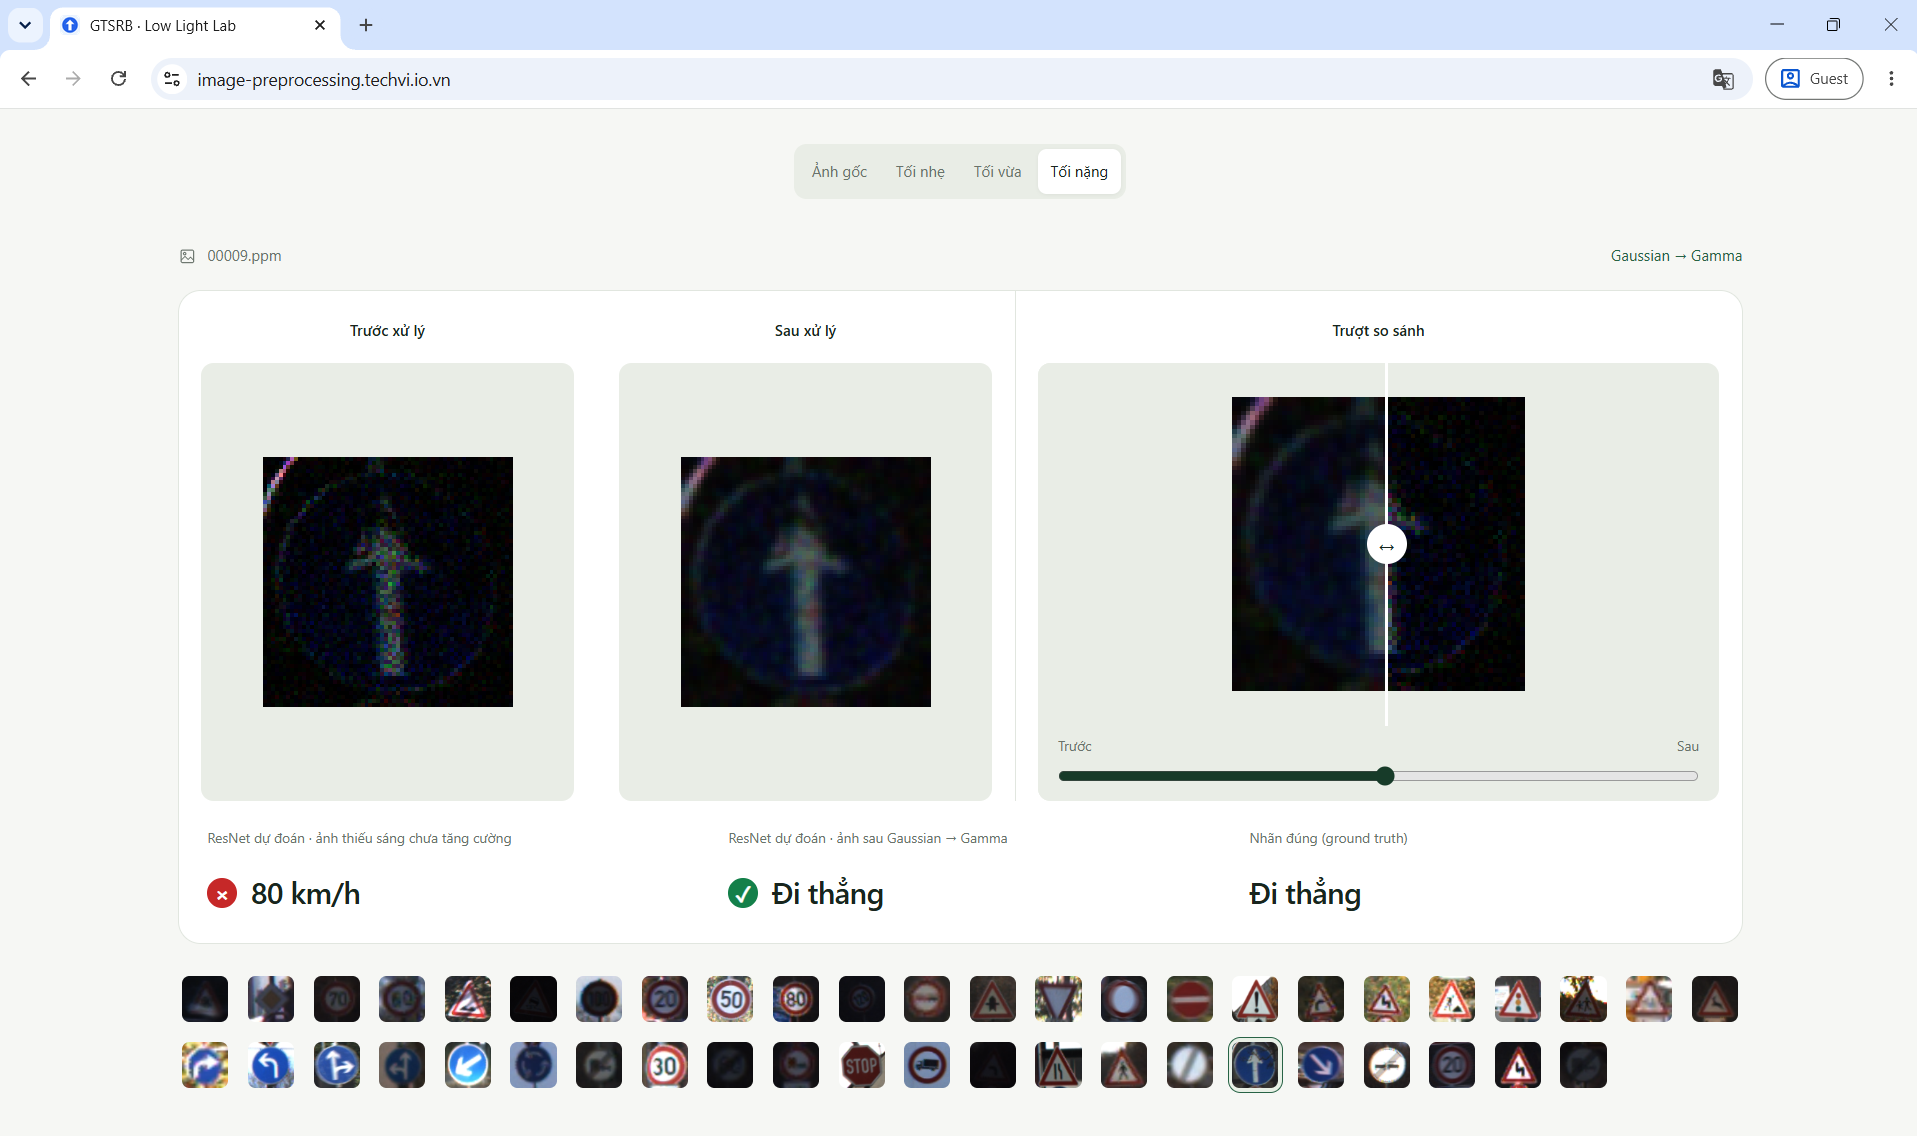
\includegraphics[width=.88\linewidth,height=4.6cm,keepaspectratio]{../latex/images/demo/website-severe.png}\par
\vspace{1mm}
{\small\href{https://image-preprocessing.techvi.io.vn}{\textcolor{Teal}{\textbf{image-preprocessing.techvi.io.vn}}}}\par
\raggedright
\textbf{Ví dụ tối nặng:} trước xử lý đoán ``80 km/h''; sau Gaussian rồi Gamma
đoán đúng ``Đi thẳng''.
\captionnote{Chọn ảnh, chọn mức suy giảm và kéo thanh so sánh. Ví dụ minh họa không thay thế kết quả toàn tập.}
\note{Bấm link để mở demo trực tiếp. Cột trái là dự đoán trên ảnh chưa xử lý, giữa là sau xử lý, phải là nhãn đúng. Mẫu 00009.ppm mức severe. Ảnh chụp do nhóm cung cấp; nguồn báo cáo mục 6.6.}
\end{frame}

\paperreference{}
\begin{frame}{6.3. Kết luận: chọn xử lý theo khả năng nhận dạng}
\textbf{Nhóm rút ra được gì?}
\begin{itemize}
\item Gaussian rồi Gamma cải thiện F1 rõ trong điều kiện tối kèm nhiễu đã mô phỏng.
\item PSNR/SSIM cao hơn không bảo đảm ResNet-18 nhận dạng đúng hơn.
\item Thứ tự xử lý phụ thuộc cấu hình; chênh lệch nhỏ chưa ổn định giữa các lần huấn luyện.
\end{itemize}
\par\vspace{2mm}
\textbf{Giới hạn và bước tiếp theo}\par
Mới kiểm tra vùng biển báo cắt sẵn và một kiến trúc phân loại.
Cần dữ liệu đêm thực có nhãn và đối chứng huấn luyện thích nghi trước khi kết luận cho camera thực tế.

\note{Đóng góp là triển khai và so sánh có kiểm soát, chưa đề xuất thuật toán mới. Không khẳng định mọi phương pháp khử nhiễu đều cần thiết hoặc mọi camera đều cải thiện. Nguồn: báo cáo chương 7.}
\end{frame}

\end{document}
